\documentclass[aspectratio=169]{beamer}
\hypersetup{colorlinks=true,allcolors=blue}
\usepackage{graphicx}
\usepackage{amsfonts,amsmath,color}       
\usepackage[spanish,activeacute]{babel}
\usepackage[utf8x]{inputenc}
\usepackage{listings}
\usepackage{fancyvrb}
%\usepackage[pdf]{pstricks}
\lstset{basicstyle=\footnotesize\ttfamily,escapeinside={\%*}{*)}}

\usefonttheme{professionalfonts}
\usetheme{Warsaw}
% Bergen, Boadilla, Copenhagen, Dresden, Hannover, Luebeck, AnnArbor, Berkeley, Darmstadt, Frankfurt, Ilmenau,     
           
% Madrid, Warsaw, Antibes, Berlin, CambridgeUS, Malmoe, PaloAlto
%\setBeamercovered{transparent}

\begin{document}



\title[PC-OS]{Introducción a la Informática: \\
Hardware, Software y Sistemas Operativos}
\author[G.R.]{Guillermo F. Rubilar}
\frame{\titlepage}

%%%%%%%%%%%%%%%%%%%%%%%%%%%

\begin{frame}
\frametitle{Contenidos}
\tableofcontents
\end{frame}

%%%%%%%%%%%%%%%%%%%%%%%%%%%

\section{Introducción}
\begin{frame}[fragile]\frametitle{Sistema Informático}
\begin{figure}
\begin{center}
\includegraphics[height=3cm]{figs/notebook.jpg}\hspace{1cm}\includegraphics[height=3cm]{figs/desktop.jpg}
\end{center}
\caption{Sistema Informático: Sistema de procesamiento de la información basado en computadores}
\end{figure}
\end{frame}

\begin{frame}[fragile]\frametitle{Computador}
\begin{itemize}
\item Máquina capaz de aceptar datos a través de un medio de entrada, procesarlos automáticamente bajo el control de un programa previamente almacenado, y proporcionar la información resultante a través de un medio de salida.
\end{itemize}
\end{frame}

\begin{frame}[fragile]\frametitle{Informática}
La Informática se ocupa de la información como materia esencial de estudio; con esta información es necesario:
\begin{itemize}
\item \textbf{Representarla} en forma eficiente y automatizable.
\item \textbf{Retransmitirla} sin errores ni pérdidas.
\item \textbf{Almacenarla} para poderla acceder y recuperar tantas veces como sea preciso.
\item \textbf{Procesarla} para obtener nuevas informaciones más elaboradas y más útiles a nuestros propósitos.
\end{itemize}
\end{frame}

\begin{frame}[fragile]\frametitle{Sistema Informático}
\begin{itemize}
\item \textbf{Hardware}: El equipo físico que compone el sistema se conoce con la palabra inglesa \textbf{hardware}, que en castellano se puede traducir como ``soporte físico". Es el conjunto de dispositivos electrónicos y electromecánicos, circuitos, cables, etc., que componen el computador.
\begin{center}
\includegraphics[height=3cm]{figs/notebook.jpg}
\end{center}
\end{itemize}
\end{frame}

\begin{frame}[fragile]\frametitle{Software}
\begin{center}

\includegraphics[height=2cm]{figs/windows-11-logo_web.png}\hfill\includegraphics[height=2cm]{figs/linux-android.jpg}\hfill
\includegraphics[height=2cm]{figs/macos-14-sonoma.png}
\end{center}
\begin{itemize}
\item \textbf{Software}: Para que el sistema trabaje, necesita que le suministren una serie de órdenes que indiquen qué es lo que queremos que haga. Estas órdenes se le suministran por medio de \textbf{programas}. El software o ``soporte lógico"\, está compuesto por todos aquellos programas necesarios para que el computador trabaje. El software dirige de forma adecuada a los elementos físicos o hardware.
\end{itemize}
\end{frame}

\section{Medidas de Información}
\begin{frame}[fragile]\frametitle{Medidas de Información}
\begin{itemize}
\item \textbf{El bit (b)} (= Binary Digit): Un elemento con \emph{dos posibles estados} en el que distinguimos \emph{dos valores} claramente diferenciados, es una variable binaria, (0 ó 1).
\item Podemos representar cualquier alfabeto en formato binario, es decir, mediante bits. Cuantos más símbolos contenga el alfabeto mayor número de bits nos harán falta para codificarlo. Hoy en día es habitual codificar tanto la información visual como la auditiva de alta fidelidad usando el \href{https://es.wikipedia.org/wiki/Sistema_binario}{sistema binario}.
\end{itemize}
\end{frame}


\begin{frame}[fragile]\frametitle{Software}

\begin{minipage}{5cm}
\begin{tabular}{c|c| c c |c|c}
Dec& Bin  & & & Dec& Bin\\ \hline
0	& 0000 & & & 8	& 1000 \\
1	& 0001 & & & 9	& 1001 \\
2	& 0010 & & & 10	& 1010 \\
3	& 0011 & & & 11	& 1011 \\
4	& 0100 & & & 12	& 1100 \\
5	& 0101 & & & 13	& 1101 \\
6	& 0110 & & & 14	& 1110 \\
7	& 0111 & & & 15	& 1111
\end{tabular}
\end{minipage}
\hfill
\begin{minipage}{5cm}
\begin{figure}
\includegraphics[height=3.5cm]{figs/Leibniz_binary_system_1697.jpg}
\caption{\href{https://es.wikipedia.org/wiki/Gottfried_Leibniz}{Gottfried Leibniz, 1697.}}
\end{figure}
\end{minipage}
\end{frame}

\begin{frame}[fragile]\frametitle{Ventajas del Sistema Binario}
\begin{itemize}
	\item Es más simple construir un dispositivo que almacene y procese información binaria, ya que sólo debe gestionar \emph{dos posibles valores/estados}.

\item Existen multitud de dispositivos con dos estados "estables" que se pueden emplear para almacenar información codificada en binario:
\begin{itemize}
	\item \textbf{Corriente eléctrica (voltaje)}: distinguir entre 10 o más niveles de voltaje es delicado y caro; distinguir entre pasa/no pasa corriente es muy simple y brinda un amplio margen de tolerancia.
	\item \textbf{Intensidad de luz}: luz apagada/luz encendida.
\end{itemize}
\end{itemize}
\end{frame}
\begin{frame}[fragile]\frametitle{Dispositivos de almacenamiento}
\begin{itemize}
	\item \textbf{Surcos en un disco óptico}.
	\begin{figure}
	\begin{center}
	\includegraphics[height=2.5cm]{figs/Discos-opticos.png}\hspace{1cm}	
	\end{center}
%	\caption{Discos ópticos.}
	\end{figure}
	\item \textbf{Perforación en papel o cartulina}.
	\begin{figure}
	\begin{center}
	\includegraphics[height=2.5cm]{figs/Used_Punchcard_(5151286161).jpg}\hspace{1cm}	
	\end{center}
%	\caption{Tarjeta perforada}
	\end{figure}
\end{itemize}
\end{frame}
\begin{frame}[fragile]\frametitle{Dispositivos de almacenamiento}
\begin{itemize}
	\item \textbf{Sentido de magnetización}: Los dispositivos magnéticos de almacenamiento usan el \textit{sentido de magnetización} de un material magnetizable.
	\begin{figure}
		\begin{center}
		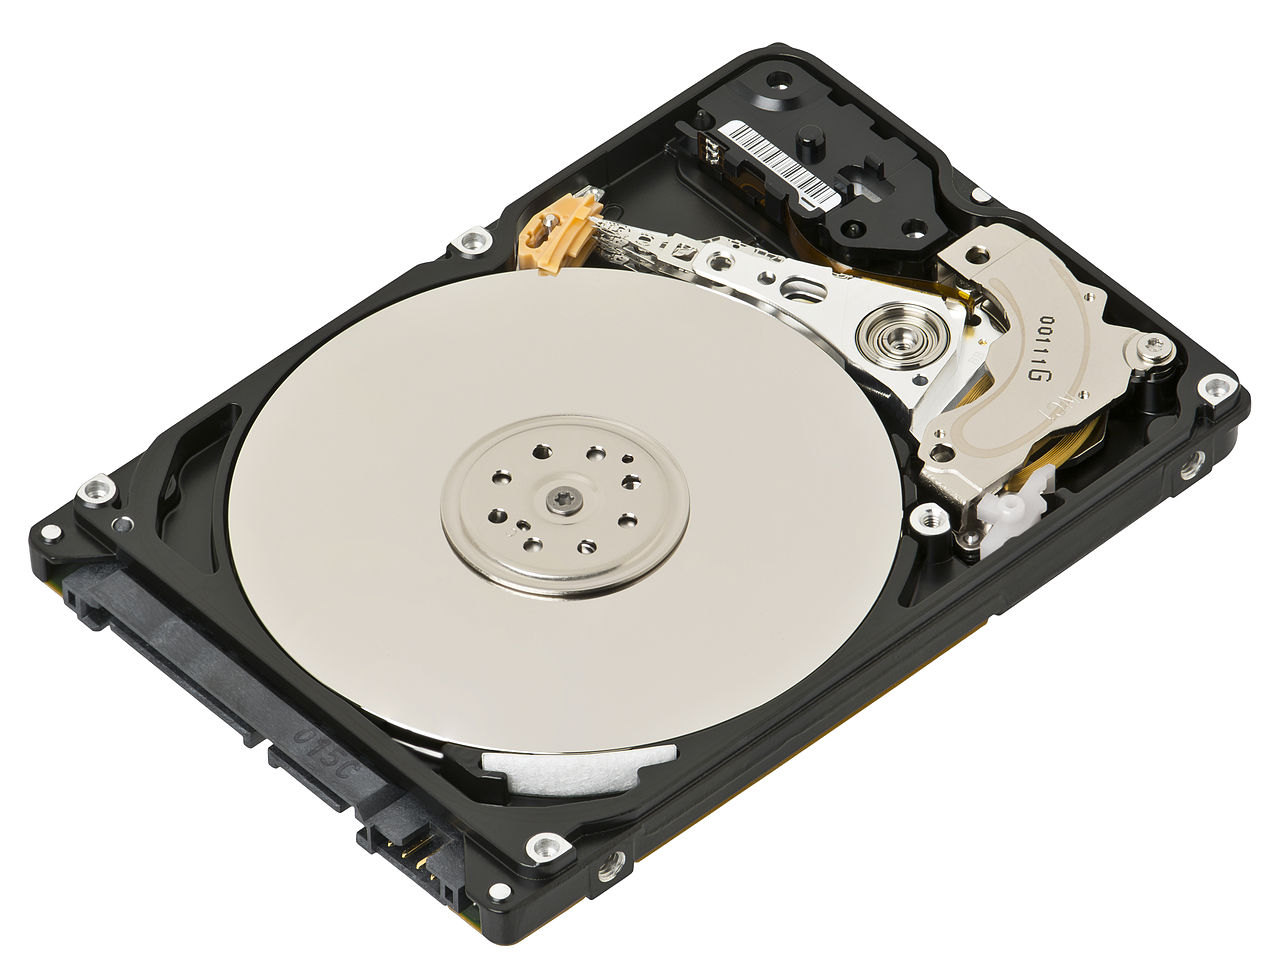
\includegraphics[height=2.7cm]{figs/1280px-Laptop-hard-drive-exposed.jpg}	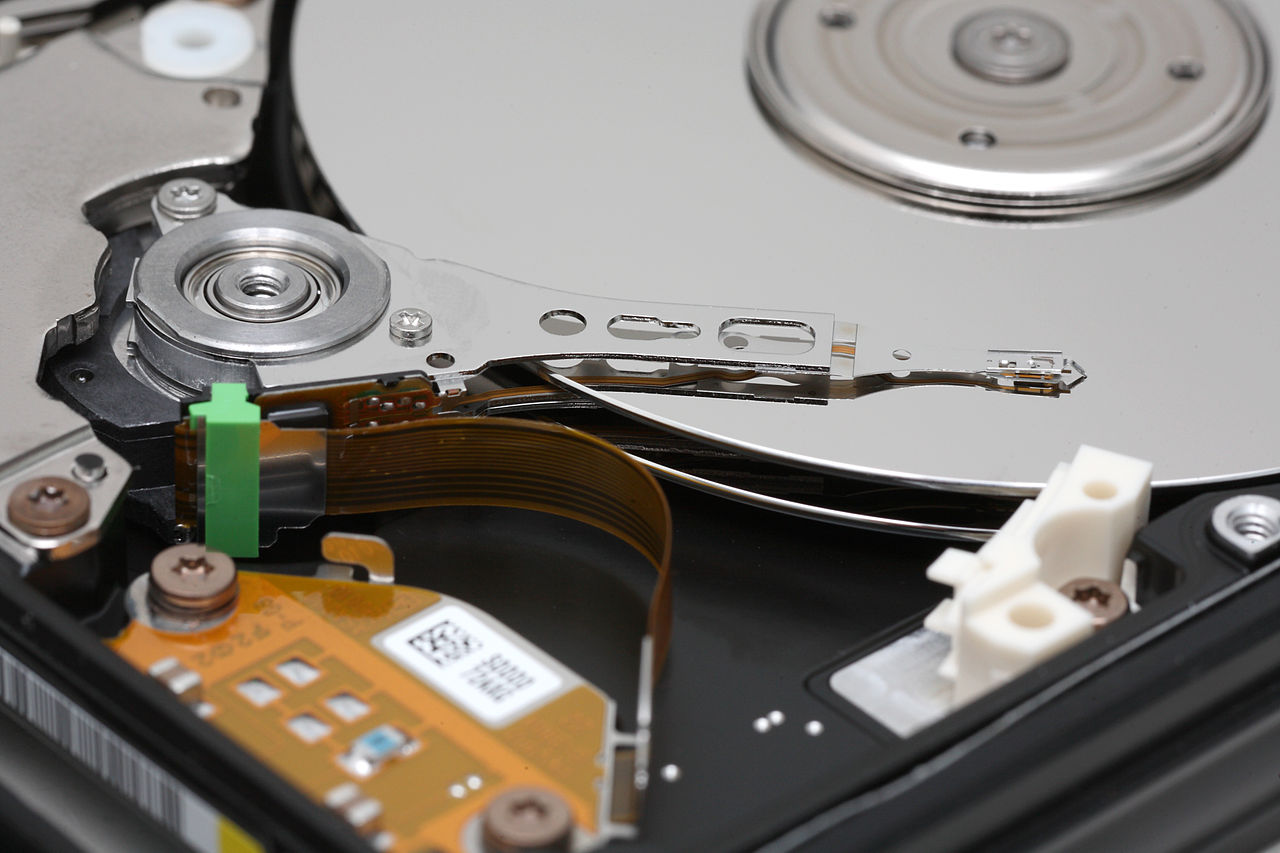
\includegraphics[height=2.7cm]{figs/1280px-Hard_disk_platters_and_head.jpg}\hspace{0.3cm}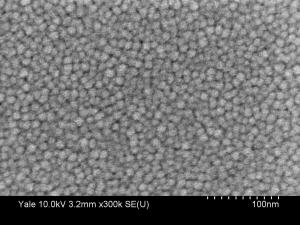
\includegraphics[height=2.7cm]{figs/HardDrivesGrainsSEM100nm-300x225.jpg}
		\end{center}
	%	\caption{Originales en https://es.wikipedia.org/wiki/Unidad_de_disco_duro y https://volga.eng.yale.edu/teaching-resources/hard-drives/methods-and-materials}
		\end{figure}
		\begin{figure}
			\begin{center}
			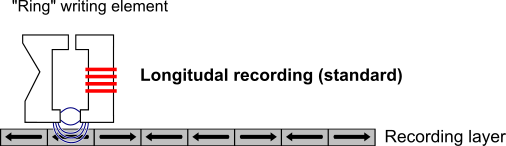
\includegraphics[height=2.5cm]{figs/Recording_Diagram.png}
			\end{center}
		%	\caption{Original en https://en.wikipedia.org/wiki/Magnetic_storage#/media/File:Perpendicular_Recording_Diagram.svg}
			\end{figure}
\end{itemize}
\end{frame}

\begin{frame}[fragile]\frametitle{Dispositivos de almacenamiento}
\begin{itemize}
	\item \textbf{SSD's}: Los péndrives, tarjetas de memoria y uidades de almacenamiento modernas \href{https://es.wikipedia.org/wiki/Unidad_de_estado_s\%C3\%B3lido}{SSD} usan  \href{https://es.wikipedia.org/wiki/Memoria_flash}{memorias flash}, basadas en diminutas (nm) ``trampas de electrones", que pueden almacenan cargas por mucho tiempo.
	\begin{figure}
		\begin{center}
		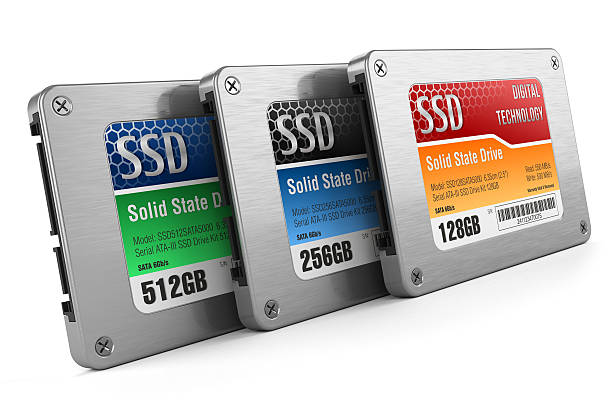
\includegraphics[height=2.7cm]{figs/ssds.jpg}\hspace{0.5cm}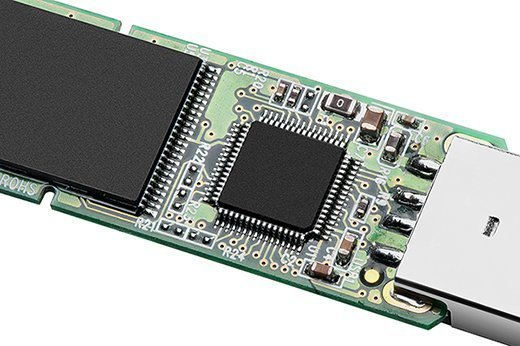
\includegraphics[height=2.7cm]{figs/nand_flash_memory_mobile.jpg}\hspace{0.5cm}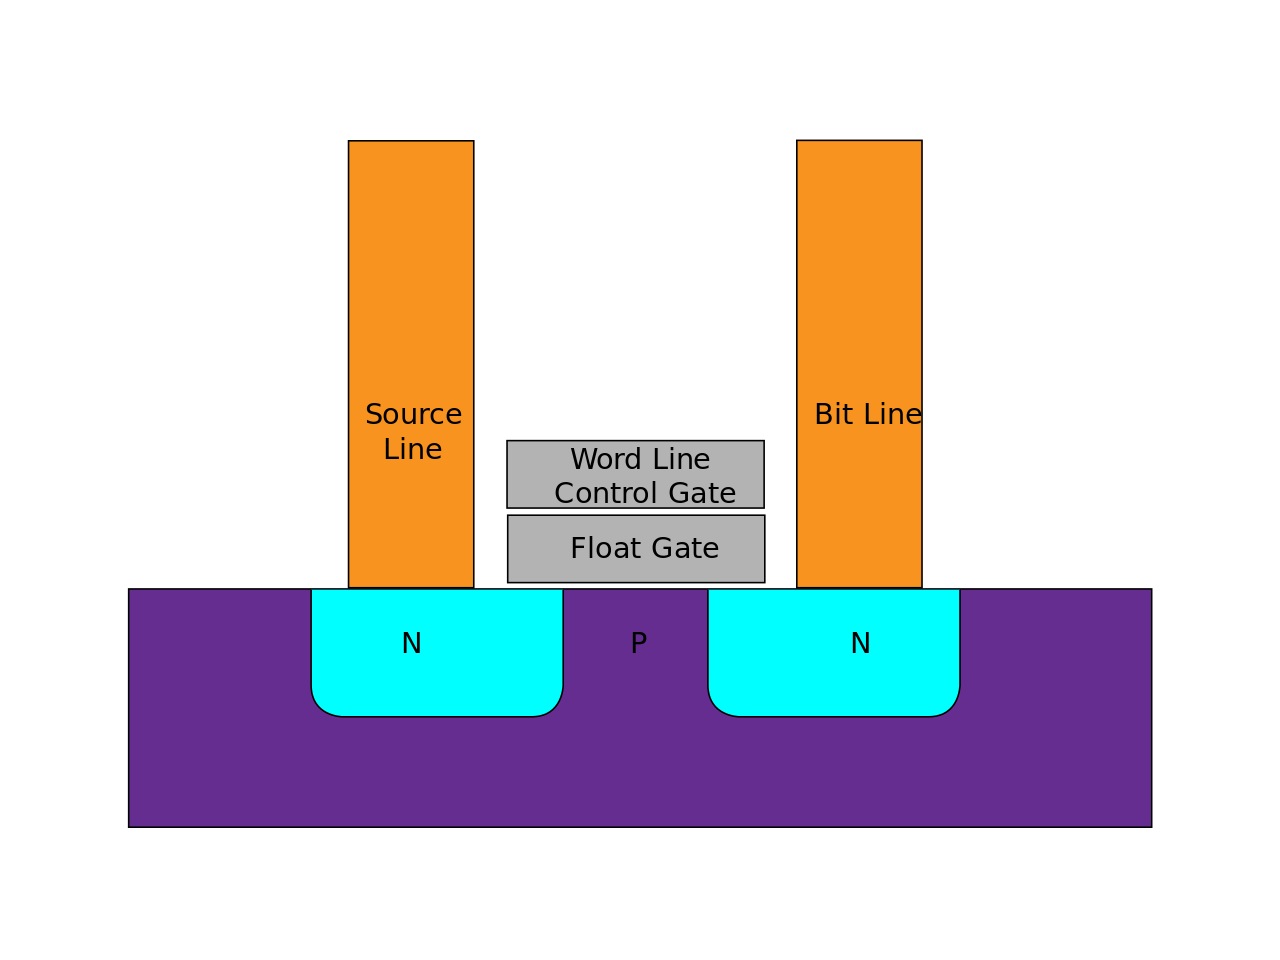
\includegraphics[height=2.7cm]{figs/Flash_cell_structure.svg.png}
		\end{center}
			\end{figure}
\end{itemize}
\begin{alertblock}{Nada es perfecto!}
Cada uno de estos dispositivos y tipos de implementación tiene sus ventajas y desventajas. Ver por ejemplo, \href{https://youtu.be/Sq3OjI3tVIM?si=Le57aclYU3NDnUOE}{este video}.
\end{alertblock}
\end{frame}

\begin{frame}[fragile]\frametitle{Medidas de Información}
\begin{itemize}
\item \textbf{El byte (B)}: El byte (típicamente) es el conjunto de 8 bits. Así, en lugar de decir que un mensaje tiene 32 bits, podemos decir que tiene 4 bytes:
$$
1 \text{B} = 8 \text{b}.
$$
Un byte puede por lo tanto adoptar $2^8=256$ estados (valores) distintos. 
\end{itemize}
\end{frame}


\begin{frame}[fragile]\frametitle{Medidas de Información: Múltiplos (k, M, G,...)}
A partir de la propuesta en de la \href{https://es.wikipedia.org/wiki/Comisi%C3%B3n_Electrot%C3%A9cnica_Internacional}{Comisión Electrotécnica Internacional} (IEC) en 1998:
\begin{itemize}
	\item \textbf{k} es la abreviatura de \textbf{kilo}, y representa un factor de multiplicación de mil, es decir $10^3$. Así que 1 kbit = 1000 bits y 1 kbyte = 1000 bytes = 8000 bits. 
	
	\item La \textbf{M} es la abreviatura de \textbf{Mega} y representa el factor de multiplicación de un millón, $10^{6}= $1.000.000.
	
	\item La \textbf{G} es abreviatura de \textbf{Giga} y representa el factor de multiplicación de mil millones, $10^{9} = $1.000.000.000.
\end{itemize}
\end{frame}


\begin{frame}[fragile]\frametitle{Medidas de Información: Múltiplos (k, M, G,...)}

\begin{block}{}
\textbf{Cuidado!:} Estas definiciones aún no son 100\% adoptadas, ya que anteriormente se prefería usar una base binaria, de modo que la definición previa a 1998 era: 1kB = $2^{10}$ B $=1024$ B, 1MB $=2^{20}$B = 1.048.576 B y 1GB $=2^{30}$B = 1.073.741.824 B, etc. 
\end{block}

\begin{block}{}
Estas viejas definiciones son ahora denotadas como kiB (kibibite), MiB (mebibyte) y  Gib (gibibyte) respectivamente. 
\end{block}
\begin{block}{}
Así, por ejemplo, 1 MiB = 1.048.576 B = 1,048576 MB.
\end{block}
Ver \url{https://es.wikipedia.org/wiki/Kibibyte} para más información.
\end{frame}

\section{Operaciones}
\begin{frame}\frametitle{Operaciones}
	\begin{center}
	\begin{tabular}{cr}
	  & CXXIII \\
	  & LXXXIV \\ \hline
	+ & CCVII\\
	\end{tabular}\hspace{2cm}
	\begin{tabular}{cr}
		& 123 \\
		& 84 \\ \hline
	  + & 207\\
	  \end{tabular}\hspace{2cm}
	  \begin{tabular}{cr}
		& 1111011 \\
		& 1010100 \\ \hline
	  + & 11001111\\
	  \end{tabular}
	\end{center}
\end{frame}	

\section{Caracteres}
\begin{frame}[fragile]\frametitle{Caracteres}
\begin{itemize}

\item \textbf{El Carácter}: Es la unidad de información \textit{a nivel del alfabeto humano}. Un carácter es, de hecho, \textit{cualquier símbolo del alfabeto usado como alfabeto normal}. Constituye una buena medida de información en términos directamente aplicables a textos expresados en el alfabeto humano.

\item Podemos clasificar los caracteres en:
	\begin{itemize}
		\item \textbf{Alfabéticos}: letras y algún que otro carácter asimilado.
		\item \textbf{Numéricos}: los dígitos numéricos del 0 al 9.
		\item \textbf{Especiales}: todos los restantes (signos de puntuación, signos monetarios, signos de operaciones aritméticas, etc).
	\end{itemize}
	\item Normalmente, en un computador, para representar un carácter se usa 1 byte de información.
\end{itemize}
\end{frame}


\begin{frame}[fragile]\frametitle{Código de caracteres ASCII}
\begin{block}{}
``\textbf{A}merican \textbf{S}tandard \textbf{C}ode for \textbf{I}nformation \textbf{I}nterchange" (= Código Estándar Estadounidense para el Intercambio de Información, 1963)
\end{block}
\begin{center}
	\includegraphics[width=5.5cm]{figs/USASCII_code_chart.png}
\end{center}
 P.ej. ``G" $\rightarrow$ [1000111] $\rightarrow$ 71, \qquad  ``$<$"$ \rightarrow$ [0111100] $\rightarrow$ 60
\end{frame}


\begin{frame}[fragile]\frametitle{Código de caracteres ASCII}
\begin{itemize}
\item Los (95) caracteres imprimibles más usados en informática:
\begin{verbatim}
  ! " # $ % & ' ( ) * + , - . / 0 1 2 3 4 5 6 7 8 9 
  : ; < = > ? @ A B C D E F G H I J K L M N O P Q R 
  S T U V W X Y Z [ \ ] ^ _ ` a b c d e f g h i j k 
  l m n o p q r s t u v w x y z { | } ~ 
\end{verbatim}
\item ASCII ordena estos caracteres asociándoles un número entre el 32 y el 126. 
\item Otros 32 caracteres no imprimibles, asociados a números 0 al 31. Representan acciones sobre el texto o el computador. P. ej, activar mayúsculas (14) o el pulsar la tecla Suprimir (127). 
\item Listado completo, $32+95 = 127$ caracteres en \href{https://es.wikipedia.org/wiki/ASCII}{Wikipedia}.

\item ASCII original no incorpora áéíóú, ni  \~n. Se crearon extensiones de 8 bits del código ASCII que incorporan estos y otros caracteres, p.ej. código \href{https://es.wikipedia.org/wiki/ISO/IEC_8859-1}{ISO 8859-1}.
\end{itemize}
\end{frame}

\begin{frame}[fragile]\frametitle{Unicode/UTF-8}
\begin{itemize}
\item Otro estándar de codificación de caracteres crecientemente popular es \href{https://es.wikipedia.org/wiki/Unicode}{Unicode}. 
\item Dise\~nado para dar soporte a múltiples lenguajes, incluyendo caracteres árabes, japoneses, chinos, griegos, y también símbolos matemáticos, técnicos, musicales y de otros tipos, incluidos emoticones! 
\item Hoy Unicode posee (versión 5.1) 100.713 caracteres, ver página oficial del \href{http://www.unicode.org/charts/}{Consorcio Unicode}, encargado de mantener y actualizar este estándar. 
\item Una de las implementaciones más populares de Unicode es la codificación \href{https://es.wikipedia.org/wiki/UTF-8}{UTF-8} (``8-bit Unicode Transformation Format'', es decir ``Formato de transformación Unicode de 8-bits"). La codificación UTF-8 es la más popular en la web.
\end{itemize}
\end{frame}


%\section{Sistema Binario}
%\begin{frame}[fragile]\frametitle{Ventajas del Sistema Binario}
%\begin{itemize}
%	\item Toda la circuitería lógica necesaria para procesar la información en binario (decodificadores, etc) es relativamente sencilla de diseñar y está sumamente estudiada.
%\end{itemize}
%\end{frame}

%\begin{frame}[fragile]\frametitle{Ventajas del Sistema Binario}
%\begin{itemize}
%	\item La aritmética en base 2 es la más fácil de implementar. Las reglas de suma, resta, multiplicación y división son las más breves y simples a la hora de construir un circuito lógico que las cumpla. Al disponer de solo dos símbolos (0 y 1), las tablas son muy simples:
%\end{itemize}
%	\begin{center}
%	\begin{tabular}{cccc}
%		 	&  	& $+$ 	& $\times$ \\ \hline
%		0 	& 0	& 0 	& 0 \\
%		0 	& 1	& 1 	& 0 \\
%		1 	& 0	& 1 	& 0 \\
%		1 	& 1	& 10 	& 1 \\
%	\end{tabular}
%	\end{center}
%\end{frame}SO

\section{Licencias de Software}
\begin{frame}[fragile]\frametitle{Licencias de Software}
\begin{block}{}
Una licencia es un \textit{contrato} que estipula los derechos y deberes de las personas que crean el software y de las personas que lo usan
\end{block}
\begin{block}{}
Típicamente, la licencia estipula bajo qué condiciones el/la usuario/a puede:
\begin{itemize}
\item Usar el software.
\item Modificar el software (requiere \textbf{código fuente}).
\item Distribuir copias del software y sus modificaciones.
\end{itemize}
\end{block}
\end{frame}

\begin{frame}
\frametitle{Licencias de Software}
\begin{block}{Tipos de Licencias}
Dependiendo de las restricciones que el/la autor/a imponga sobre cada uno de estos tres aspectos, es posible clasificar un determinado software en dos grandes grupos:
\begin{itemize}
\item \textbf{Software Propietario}: El/la autor/a restringe alguno de los aspectos anteriores. P.ej. permite el uso gratuito del software y su distribución, pero no su modificación (Freeware).
\item \textbf{Software Libre}: El/la autor/a permite tanto el uso y la modificación del software, así como la distribución de copias.
\end{itemize}
\end{block}
Para más información, ver artículo en \href{https://es.wikipedia.org/wiki/Licencia_de_software}{Wikipedia}.
\end{frame}
\end{document}